\section{Definition von SIEM}

\gls{SIEM} ist das Ergebnis von der Kombination zwischen \glsfirst{SEM} und \glsfirst{SIM} \citep{Dorigo_SIEM}. Das erste bezieht sich auf der Identifizierung, Bewertung, Beobachtung und Bericht von Sicherheitsvorfällen mithilfe von verschiedenen Logdateien \citep{techopedia_SEM}. Das zweite ist ein Software, der bei der automatischen Sammlung von Loginformationen aus vielen Quellen, wie Firewall und Servers, untersützt \cite{techopedia_SIM}. 

In dem Universum von \glsfirst{SOC} mischen sich verschiedenen Begriffe, die manchmal zur Verwirrung führen, weil sie ähnliche Bedeutung und Verantwortung haben. \glsfirst{IDS}, \glsfirst{IPS} und \glsfirst{SIEM} werden von \textit{nonnative users} und sogar von Spezialisten oft verwechselt, da ihre Aufgabe mehr Zusammenhang als Unterschied haben. Um Umfang dieser Arbeit wegen der zeitlichen Einschränkungen zu verringen, fassen wir kurz die Unterschiede zwischen ihnen zusammen und legen wir unsere Grenze auf den \glspl{SIEM} Lösungen fest.

\glsfirst{IDS} sind Software oder Hardware die \glsplural{Cyberangriff} identifzieren und berichten. Sie haben eine passive Rolle, weil sie die \glsplural{Cyberangriff} weder stoppen noch verhindern können. \glsfirst{IPS} seinerseits haben eine aktive Haltung gegenüber \glsplural{Cyberangriff}, die können automatisch behandeln, indem sie Blocking-Mechanismus einschalten, um den Angriff zu stoppen \citep{Wendzel_IS}. Wie \gls{IDS}, kann der \gls{IPS} auch Logdateien generieren, die von einer \gls{SIEM} Lösung gesammelt werden kann. 

Die beiden ersten können innerhalb eines Unternehmen coexistieren, müssen aber nicht. Die Datenquellen von \glsplural{SIEM} können, unter anderen, von diesen beiden Tools entstehen. Die folgenden Abbildung stellt didaktisch, wie sich \glsplural{SIEM} in diesem Landschaft integrieren lassen: 

\begin{figure}[H]
   \centering
   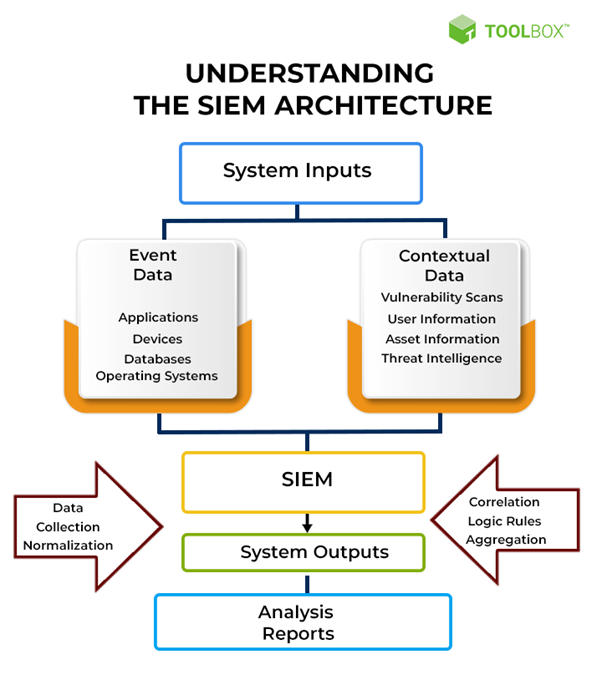
\includegraphics[width=0.8\textwidth]{assets/2_p1.png}
   \caption{Allgemeine Informationsfluss von \gls{SIEM} \\Quelle: \citep{Mohanan_What} }
   \centering
\end{figure}

Aus dem Bild können wir feststellen, dass \glsplural{SIEM} für die Zentralisierung von Sicherheitsdaten zuständig ist. Diese werden dann bearbeitet und in einem oder mehreren Berichten dargestellt, damit das \gls{SOC}-Team schnellere und effektive Entscheidungen treffen können. Der Informationsfluss einer \gls{SIEM} Lösung können wirder in der folgenden Abbildung darstellen:

\begin{figure}[H]
   \centering
   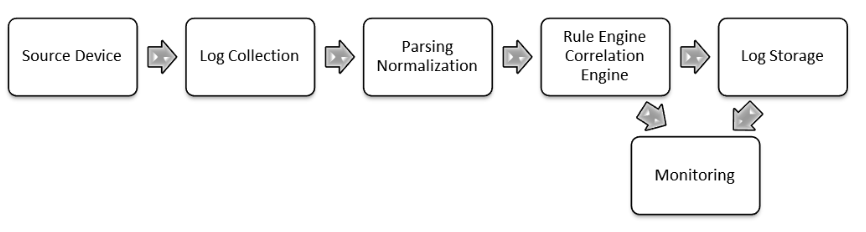
\includegraphics[width=0.8\textwidth]{assets/2_p2.png}
   \caption{Allgemeine Informationsfluss von \gls{SIEM} \\Quelle: \citep{Granadillo_SIEM} }
   \centering
\end{figure}

\gls{SIEM} ist aber viel mehr als eine Sammlung von Logdateien. Das Ziel dieser Software ist die automatische Analyse zu ermöglichen, indem Daten kombiniert und bewertet werden können. In vielen Bereiche, wie Finanzen (\glsfirst{PCDISS}), Gesundheitswesen (\glsfirst{HIPAA}), sind \glsplural{SIEM} gesetzliche Verpflichtung \citep{Jog_SIEM}. In Deutschland verplichtet das \gls{IT-Sicherheitsgesetz 2.0} Organisationen mit kritischen Infrastrukturen die Anwendungen von solche Lösungen, um Störungen der \glsfirst{CIA} zu verhindern \citep{BSI_ITSG}.

\subsection{Existierende SIEM Lösungen}

Die existierenden \glsplural{SIEM} Lösungen können in zwei Kategorie getrennt werden: \textit{\gls{Proprietary}} und \textit{\gls{Open Source}}. Zu der ersten ist Splunk von dem Unternehmen Splunk Technology die meist verwendete Software \citep{Kazarov_Splunk}. Da unser Fokus hier auf \textit{\gls{Open Source}} Lösungen liegt, diskutieren wir hier demnächst über folgende Software:

\textbf{\textcolor{red}{Wie konnte ich Grafana hier erwähnen? Grafane ist eher algemmein und nicht so zu Alert orientiert, habe ich hier gefunden: \href{https://www.metricfire.com/blog/grafana-vs-splunk/}{Splunk x Grafana} und hier \href{https://www.researchgate.net/publication/350730340_Implementation_of_Grafana_as_open_source_visualization_and_query_processing_platform_for_data_scientists_and_researchers}{What is Grafana}}  }

\begin{itemize}[noitemsep]
   \item Prelude
   \item AlienVault \glsfirst{OSSIM}
   \item ELK Stack
\end{itemize}

\subsubsection{Prelude}
Das im Jahr 2002 in Frankreich von Yoann Vandoorselaere freigegebene Tool Prelude zählt zu gehört zu einer europäischen \gls{Open Source} \gls{SIEM} Lösung. Laut dem Anbieter verfügt Prelude unter anderen folgenden Funktionalitäten \citep{Prelude_SIEM}:

\begin{itemize}[noitemsep]
   \item Informationszentralisierung
   \item Datenaggregation und -Zusammenhang mit vordefinierten und von den Nutzer angepassten Regeln 
   \item Einbruchserkennungmechanismen
   \item Datennormalisierung
\end{itemize}

Die Anwendung besteht aus verschiedenen unabhängige Modulen. Unter denen highlighten wir folgende: Warnmeldung, Archivierung, Analyse und Verwaltung. Das erste gehört zu der zentrallen Aufgabe dieser Lösung, es ist dafür zuständig, Daten zu empfangen, zu normalisieren, Zusammenhang zu machen und Meldungen zu generieren. Das zweite Modul, Archivierung, konzentriert sich auf die Speicherung und Verfügbarkeit der Daten. Zu der Analyse-Modul gehören statistische Aufgabe und Darstellung in verschiedenen Formaten. Das letzte Modul dient dazu, die Anwendung zu steuern, Nutzer zu erstellen dessen Rechts zu konfigurieren \citep{EC_Prelude}.

Die wissenschaftliche Literatur über Prelude ist sehr eingeschränkt. Wenige Publikationen fokussieren sich auf die Entwicklung, Implementation und unternehmerische Anwendung dieses Tools. Eine Studie von 2021 versuchte dieses und zwei andere Tools (AlienVault und Cyberoam iView) anhand technischer und nutzerfreundliche Kriterien zu vergleichen. Unter diese Kriterien highlighten wir folgende \citep{Grammatikis_Prelude}:

\begin{itemize}[noitemsep]
   \item \textbf{technische Kriterien}
   \begin{itemize}[noitemsep]
      \item Real-time performance, 
      \item Range and flexibility of reporting
      \item Alert correlation
   \end{itemize}

   \item \textbf{nutzerfreundliche Kriterien}
   \begin{itemize}[noitemsep]
      \item Documentation comprehensiveness
      \item Complexity of the installation process
      \item Complexity of the system configuration
   \end{itemize}
\end{itemize}

In den technische Kriterien lag Prelude an dritten Platz und in den nutzerfreundliche Kriterien bekam Prelude den ersten Platz. 

Auch in den nicht wissenschaftlichen Publikationen existieren begrenzte Anzahl von Texten über Preludes. Die existierenden kommentieren ganz zusammenfassend über die ausreichende Dokumentation und heben hervor, dass es eher eine in Europa konzentrierte Lösung.

\subsubsection{AlienVault OSSIM}
AlienVault OSSIM ist eine im Jahr 2007 entwickelte \gls{Open Source} SIEM Lösung. Im Jahr 2018 wurde sie von der Firma AT\&T Communication gekauft \citep{CBN_AV}. In der Beschreibung des Anbieters steht, dass sie auch dabei untersützt, Daten zu sammeln, zu normalisieren und zu bewerten. Er behaupt auch, dass sein Tool in der Lage ist, Schwachstelle und Angriffe zu erkennen, Verhältnis zu beobachten und Datenzusammenhang durchzuführen \citep{ATT_AVO}.

Laut der Website Comparitech steht AlienVault in der 13ten Platz von den besten bewerteten \gls{SIEM} Lösungen. Die Seite beschreibt auch, dass einen \gls{IDS}, Verhaltensüberwachungssystem und einen Schwacstellescanner integriert sind . Die Anwendung ist auch mit der Platform \gls{OTX} verbunden, diese ermöglicht die Teilung von Informationen über Schwachstelle. Comparitech highlighted, dass die Anwendung wegeren ihre nidriegen Kosten besser für kleine oder mittelständige Unternehmen geignet ist \citep{comparitech_SIEM}. 

Die Anwendung bietet konsitente Datenzusammenhang von Daten und vermeidet den Auftauch von \gls{falsch positiv}. AlienVault kommt auch mit vordefinierten Use-Cases, die dabei unterstützen gewöhnlichen Angriffsszenario zu erkennen. Die Installation, die Einstellung und die Integration mit anderen Tools ist auch benutzerfreundlich \citep{Gomes_AV}. Aus einer anderen wissenschaftlicher Quelle fanden wir heraus, dass es für viele  Quelle eine manuelle Normalisierung der Logdatein notwendig ist \cite{Nabil_AV}. Die Anwendunt hat aber einen zuverlässigen Berichtsmechanismus.

\subsubsection{ELK Stack}
cccccccccc

\subsubsection{Zusammenfassender Vergleich}
ddddddddd

\subsection{Auswahlkrietieren}
Für diese haben entschieden wir uns für die XXXXX \gls{SIEM} Lösung aus folgenden Grunden:

\begin{itemize}[noitemsep]
   \item eingeschränkte Ressource für die Entwicklung dieser Arbeit
   \item bbbbbbbbbbbbbbb
   \item ccccccccccccccc
   \item ddddddddddddddd
   \item eeeeeeeeeeeeeee
\end{itemize}

Demnächst fokussieren wir uns in der Installation, Konfiguration und Implementation von XXXXXX. Danach werden wir spezifische Logdateiein der Hochschule importieren, normalisieren und diese anhand Angriff1 und Angriff2 beobachten.